\section{Einführung}
Ein Hopfield Netzwerk ist eine spezielle Art eines künstlichen neuronalen Netzwerkes. Ziel des Hopfield Netzes ist die assoziative Speicherung von Mustern. Dies bedeuted, dass Speicherinhalt nicht über eine Speicheradresse erreicht werden soll, sondern dass das Netzwerk auf ein Eingabemuster mit dem gespeicherten Muster antwortet, welches die größte Ähnlichkeit aufweist. Hopfield-Netze können somit genutzt werden, um ein verrauschtes oder nur in Teilen vorhandenes Muster zu rekonstruieren. Dies könnte natürlich auch über die serielle Berechnung der Abstände des Eingabemusters zu den gespeicherten Mustern realisiert werden. Hierbei geht es aber darum die genannte Funktionsweise durch ein neuronales Netz zu implementieren.

\subsection{Netzwerkstruktur}
Das Hopfield Netz besteht aus einer einfachen Schicht von Neuronen $S_i$, welche binäre Werte annehmen können. Jedes Neuron ist mit jedem anderen Neuron verbunden. Diese Verbindung ist durch die symmetrischen Gewichte $w_{ij} = w_{ji}$ gegeben. Mit jedem Zeitschritt evolviert das Netz gemäß der McCulloch-Pitts Gleichung
\begin{align}
S_i(t+1) =  sgn(\sum_j w_{ij} S_j(t) - \theta_i) ,
\end{align}
welche zur Minimierung der Energiefunktion
\begin{align}
H = - \frac{1}{2} \sum_{ij} w_{ij} S_i S_j + \sum_{i} \theta_i S_i
\end{align}
führt.

Die Aktualisierung des Netzes kann dabei über synchron oder asynchron erfolgen. Wird das Hopfield Netz asynchron aktualisiert, ist garantiert, dass Konvergenz erreicht wird, da $H$ im jedem Schritt kleiner wird oder gleich bleibt. Im synchronen Modus kann es zu sogenannten Oszillationen kommen. Die Ursache für diese sowie die Vorteile/Nachteile der beiden Update-Modi werden in Aufgabenteil 4.2 diskutiert.

\subsection{Speichern von Mustern}
Mithilfe der Hebb'schen Lernregel können Muster im Netzwerk gespeichert werden:
\begin{align}
w_{ij} = \frac{1}{N}\sum_{\mu = 1}^{p} xi_i^{(\mu)} xi_j^{(\mu)}
\end{align}

\subsection{Spurious states}
Zusätzlich zu den gespeichterten Bildern kommt es zu weiteren Nebenminima, den sogenannten \textbf{spurious states}. Diese lassen sich in drei Kategorien unterteilen:
\begin{itemize}
\item Erstens ist auch das Negative jedes Bildes ein Minimum (\textbf{reversed states}).
\item Zweitens ist auch jede ungerade Linearkombination von Bildern (\textbf{mixture states}) ein Nebenminimum:
\begin{align}
\bar{\xi}_i^{\textup{mix}} = sgn(\pm \xi_i^{(\mu_1)} \pm \xi_i^{(\mu_2)} \pm \xi_i^{(\mu_3)} \pm \dots)
\end{align}
\item Drittens kann es bei großen $p$ zu lokalen Minima kommen, die weder eine Linearkombination noch anders korreliert zu den gespeicherten Bildern sind (\textbf{spinglass states}).
\end{itemize}
Da die \textbf{spurious states} im Mittel einen relativ kleinen \textbf{basin of attractions} besitzen , kann das Hopfield Netz dennoch als Assoziativspeicher genutzt werden.




\subsection{Endliche Temperaturen}
Um die Wahrscheinlichkeit in ein Nebenminima zu konvergieren zu verringern, gibt es die Möglichkeit ein sogenanntes stochastisches Rauschen in die deterministishen McCulloh-Pitts Gleichung einzuführen. Diese sogenannten endlichen Temperaturen können dazu führen, dass die erreichten Nebenminima überwunden werden und in eines der gespeicherten Bilder konvergiert werden. Allerdings führen  die endlichen Temperaturen auch dazu, dass keine exakte Konvergenz mehr erreicht werden kann, da immer eine Fluktuation möglich ist.

\begin{figure}[htp]
	\centering
	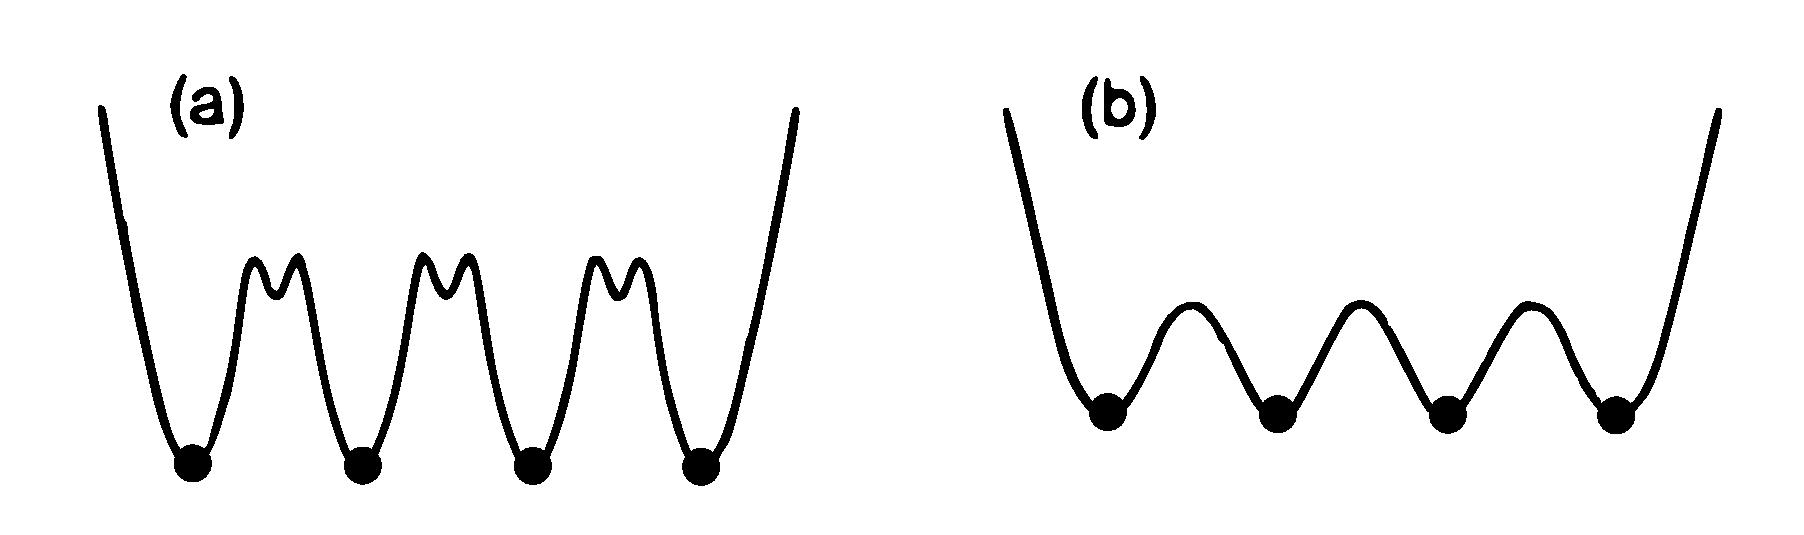
\includegraphics[width = 0.7\textwidth]{images/spurious_states_and_finite_temperature.pdf}
	\caption{Schematische Darstellung der \textbf{energy landscapes} für $p << N$. (a) Die mixture states können sich als lokale Minima zwischen den gespeicherten Bildner vorgestellt werden. Die eigentlichen Zustände sind natürlich Eckpunkte im $N$-dimensionalen Hyperwürfel. (b) Bei hoher Temperature verschieden die "mixture states". (Quelle: \cite{hertz_krogh_palmer})}
	\label{fig:spurious_states_and_finite_temperature}
\end{figure}


Zur Vorbereitung die wurden \cite{bunk} und \cite{hertz_krogh_palmer} herangezogen.


\clearpage